\documentclass[11pt,a4paper]{article}

% --- geometry and fonts -----------------------------------------------
\usepackage[margin=2.5cm]{geometry}
\usepackage[T1]{fontenc}
\usepackage[utf8]{inputenc}
\usepackage[english]{babel}

% --- math -------------------------------------------------------------
\usepackage{amsmath}
\usepackage{amssymb}
\usepackage{amsfonts}
\usepackage{mathtools}
\usepackage{siunitx}
\numberwithin{equation}{section}

% --- tables -----------------------------------------------------------
\usepackage{enumitem}
\usepackage{booktabs}
\usepackage{tabularx}
\usepackage{longtable}   % page-spanning per-corpus metric tables
\newcolumntype{L}{>{\raggedright\arraybackslash}X}
\newcolumntype{C}{>{\centering\arraybackslash}X}
\newcolumntype{R}{>{\raggedleft\arraybackslash}X}

% --- figures and captions ---------------------------------------------
\usepackage{graphicx}
\graphicspath{{figures/}}
\usepackage[font=small,labelfont=bf]{caption}
\usepackage{subcaption}
\usepackage{float}
\usepackage{rotating}   % sidewaystable for the wide per-surface table

% --- algorithms -------------------------------------------------------
\usepackage[ruled,vlined]{algorithm2e}

% --- theorem-like environments ----------------------------------------
\usepackage{amsthm}
\newtheorem{principle}{Principle}[section]
\newtheorem{definition}{Definition}[section]
\newtheorem{property}{Property}[section]
\newtheorem{proposition}{Proposition}[section]

% --- tikz / pgfplots --------------------------------------------------
\usepackage{tikz}
\usetikzlibrary{
  fit, shapes, calc, positioning, arrows, arrows.meta,
  shapes.multipart, decorations.markings, backgrounds
}
\usepackage{pgfplots}
\pgfplotsset{compat=1.18}

% --- shared figure palette + styles -----------------------------------
% The rapidfem/rapidmesh palette (kept in sync with site/src/lib/theme.ts) is
% defined for the colour figures only, the rendered MESH figures and any data
% PLOTS (pgfplots cycle below). The schematic flow diagrams are deliberately
% PLAIN black-and-white line art (no fills, no colour), classic-academic.
\definecolor{rmaccent}{HTML}{D9513C}   % lava
\definecolor{rmamber}{HTML}{E8944A}    % amber
\definecolor{rmgreen}{HTML}{6BBF8A}    % green
\definecolor{rmpurple}{HTML}{7B5E8A}   % purple
\definecolor{rmblue}{HTML}{4A9EC2}     % blue
\definecolor{rmolive}{HTML}{C4C46B}    % olive
\pgfplotscreateplotcyclelist{rm}{%
  {rmaccent},{rmamber},{rmgreen},{rmpurple},{rmblue},{rmolive}}
% rapidmom report style: accent the caption labels (Figure/Table N).
\captionsetup{labelfont={bf,color=rmaccent}}
% Plain black-and-white diagram styles (white fill, black stroke, black text).
\tikzset{
  >={Stealth[length=4.5pt]},
  rm edge/.style={draw=black, ->, line width=0.6pt},
  rm flow/.style={draw=black, ->, line width=0.8pt},
  rm op/.style={draw=black, fill=white, circle, minimum size=7mm, inner sep=1pt,
    font=\small, line width=0.6pt},
  rm state/.style={draw=black, fill=white, rounded corners=2pt, inner sep=3pt,
    font=\small, line width=0.6pt},
  rm param/.style={draw=black, fill=white, rounded corners=2pt, inner sep=3pt,
    font=\small, line width=0.6pt},
  rm sel/.style={draw=black, fill=white, diamond, aspect=2, inner sep=1pt,
    font=\footnotesize, line width=0.6pt},
  rm stage/.style={draw=black, fill=white, rounded corners=3pt, align=center,
    font=\small, minimum height=10mm, text width=24mm, line width=0.7pt},
  rm out/.style={draw=black, fill=white, rounded corners=3pt, align=center,
    font=\small, minimum height=10mm, text width=24mm, line width=0.7pt},
  rm hi/.style={draw=black, line width=1pt},
}

% --- macros -----------------------------------------------------------
\newcommand{\R}{\mathbb{R}}
\newcommand{\norm}[1]{\left\lVert #1 \right\rVert}
\newcommand{\abs}[1]{\left\lvert #1 \right\rvert}
\newcommand{\vv}[1]{\mathbf{#1}}
\newcommand{\dd}{\,\mathrm{d}}
\newcommand{\Su}{\vv{S}_u}
\newcommand{\Sv}{\vv{S}_v}
\DeclareMathOperator{\proj}{proj}
\DeclareMathOperator{\dist}{dist}
\newcommand{\T}{\mathsf{T}}
\DeclareRobustCommand{\code}[1]{\texttt{#1}}
\setlength{\emergencystretch}{3em}

% --- citations --------------------------------------------------------
\usepackage{csquotes}
\usepackage[backend=biber, style=ieee, sorting=none]{biblatex}
\addbibresource{references.bib}

% --- links (last) -----------------------------------------------------
\usepackage[
  pdftitle={rapidmesh: Hierarchical Bottom-Up Variational Meshing},
  pdfauthor={rapidmesh},
  colorlinks=true, linkcolor=rmaccent, citecolor=rmaccent, urlcolor=rmblue
]{hyperref}
\usepackage[noabbrev]{cleveref}
\crefname{principle}{Principle}{Principles}
\Crefname{principle}{Principle}{Principles}
\crefname{algocf}{Algorithm}{Algorithms}
\Crefname{algocf}{Algorithm}{Algorithms}

\title{\textbf{\textcolor{rmaccent}{rapidmesh}}\\[2pt]
\large A Pure-Rust Hierarchical Mesher for B-Rep Solids:\\
\large Conforming Tetrahedra, Sliver-Free Surfaces, FEM/MoM Export}
\author{Milan Rother}
\date{\today}

\begin{document}
\maketitle

\begin{abstract}
This document specifies the meshing algorithm rapidmesh uses to turn a
boundary representation (B-Rep) of one or more material regions into a
conforming, isotropic, high-quality tetrahedral mesh. The algorithm is
\emph{dimensionally hierarchical}: it meshes $0$-cells (corners), then $1$-cells
(edges), then $2$-cells (faces), then the $3$-cell (volume), and \emph{freezes}
each level before the next consumes it. Within every dimension it combines
\emph{error-driven adaptive sampling} (insert where a geometric tolerance is
violated) with \emph{variational point relaxation} for quality---a sizing-weighted
centroidal-Voronoi (Lloyd) relaxation on edges and faces, and an
\emph{optimal-Delaunay} (ODT) relaxation in the volume. The frozen surface
triangulation is a
\emph{hard constraint} on the volume Delaunay, which is what makes the boundary
watertight by construction. We derive, with a computer-algebra system, the
arc-length, curvature, deflection-sizing, first/second fundamental form and
distance-faithful chart formulae for every edge and face modality the geometry
kernel supports (line, circle/arc, surface--surface intersection, NURBS curve,
extruded profile; plane, cylinder, cone, sphere, torus, extruded/ruled, NURBS),
and give pseudocode for each stage.
\end{abstract}

\clearpage
\tableofcontents
\clearpage
\listoffigures
\clearpage
\listoftables
\clearpage

% ============================================================================
\section{Design philosophy}
% ============================================================================

\begin{principle}[Dimensional hierarchy]
A $k$-cell is meshed only after every $(k{-}1)$-cell on its boundary is meshed
and \emph{frozen}. Corners pin edges; edges pin faces; faces pin the volume.
Shared lower-dimensional entities are meshed once and reused, so adjacent
cells agree on their common boundary exactly (conformity across seams is
inherited, not reconstructed).
\end{principle}

\begin{principle}[Two orthogonal mechanisms per level]
Each dimension uses (i) \emph{error-driven adaptivity} to decide \emph{how many}
points and \emph{where} (insert at the worst geometric-error location, then
re-relax, until a tolerance is met), and (ii) \emph{variational relaxation} to
decide \emph{point quality} --- a density-weighted centroidal-Voronoi (Lloyd) move
on edges and faces, and the optimal-Delaunay (ODT) move \eqref{eq:odt} in the
volume. Adaptivity controls density; the relaxation controls regularity.
\end{principle}

\begin{principle}[Constrained volume, not recovered boundary]
The frozen surface triangulation enters the volume stage as a set of
\emph{constraint facets}. The volume tetrahedralization is required to contain
them as faces. The boundary is therefore \emph{enforced}, not statistically
recovered: there are no straddling tetrahedra, hence no ``noses'' protruding
into a void and no gaps. The surface is therefore completed \emph{before} the
volume is seeded.
\end{principle}

\begin{principle}[Embarrassingly parallel within each level]
\label{prin:parallel}
Freezing a level before the next consumes it makes the entities \emph{within} a
level mutually independent: they share only already-frozen, read-only
lower-dimensional boundary. Hence each level is processed in parallel with no
synchronisation:
\begin{itemize}[topsep=2pt,itemsep=1pt]
\item \textbf{all edges} at once (each depends only on its two fixed corners);
\item then \textbf{all faces} at once (each depends only on its fixed boundary
edges, which are computed once and read concurrently);
\item then \textbf{all volume regions} at once (each material region's
constrained tetrahedralization depends only on its fixed bounding surface;
shared interface facets are read-only).
\end{itemize}
Shared lower-dimensional entities are meshed exactly once and cached, which is
what removes write contention. Each entity's result is independently
deterministic and merged in fixed id order, so parallelism does not affect
reproducibility (\cref{sec:notation}). The three barriers (edges $\to$ faces
$\to$ volume) are the only synchronisation points.
\end{principle}

\noindent
The geometry source is a B-Rep assembled from the exact CSG arrangement: faces
are trimmed analytic (or NURBS) surfaces, edges are analytic curves (including
the intersection curves booleans create), vertices are corner points, and the
radial-edge topology records which faces meet along each edge and the material
region on each side. The mesh is built \emph{from this geometry}, independent of
any input tessellation. \Cref{fig:pipeline} shows the whole pipeline.

\begin{figure}[H]\centering
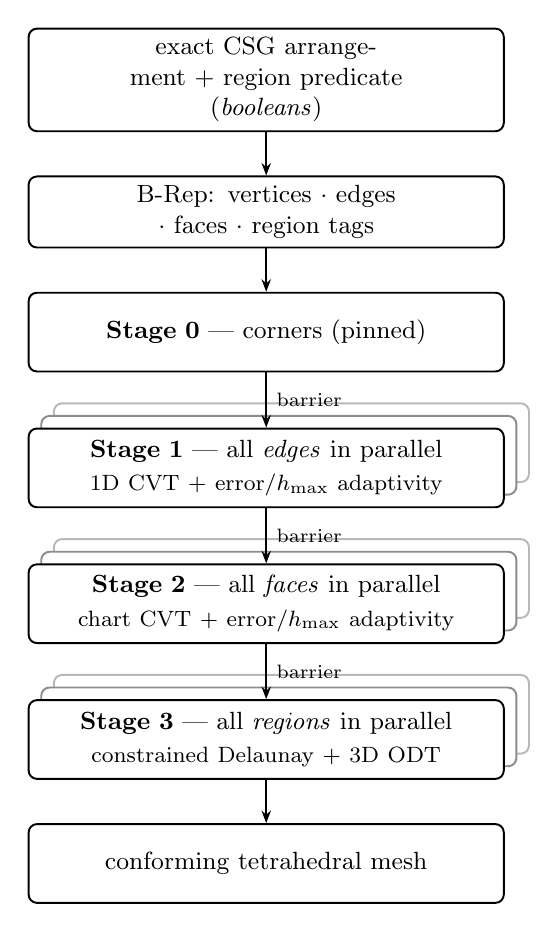
\begin{tikzpicture}[font=\small, node distance=5.5mm,
   stg/.style={rm stage, text width=58mm, align=center},
   pre/.style={draw=black, fill=white, rounded corners=3pt, text width=58mm,
     align=center, minimum height=9mm, font=\small, line width=0.7pt}]
 \node[pre] (csg) {exact CSG arrangement $+$ region predicate \\ (\emph{booleans})};
 \node[pre, below=of csg] (brep) {B-Rep: vertices $\cdot$ edges $\cdot$ faces $\cdot$ region tags};
 \node[stg, below=of brep] (s0)
   {\textbf{Stage 0} — corners (pinned)};
 \node[stg, below=7mm of s0] (s1)
   {\textbf{Stage 1} — all \emph{edges} in parallel\\[1pt]
    {\footnotesize 1D CVT $+$ error/$h_{\max}$ adaptivity}};
 \node[stg, below=7mm of s1] (s2)
   {\textbf{Stage 2} — all \emph{faces} in parallel\\[1pt]
    {\footnotesize chart CVT $+$ error/$h_{\max}$ adaptivity}};
 \node[stg, below=7mm of s2] (s3)
   {\textbf{Stage 3} — all \emph{regions} in parallel\\[1pt]
    {\footnotesize constrained Delaunay $+$ 3D ODT}};
 \node[rm out, below=of s3, text width=58mm, align=center] (mesh)
   {conforming tetrahedral mesh};
 \begin{scope}[on background layer]
   \foreach \n in {s1,s2,s3}{
     % far shadow first (bottom), near shadow on top of it, main node on top
     \node[stg, draw=black!28, fill=white] at ([shift={(3.2mm,3.2mm)}]\n.center){};
     \node[stg, draw=black!45, fill=white] at ([shift={(1.6mm,1.6mm)}]\n.center){};
   }
 \end{scope}
 \draw[rm flow] (csg)--(brep);
 \draw[rm flow] (brep)--(s0);
 \draw[rm flow] (s0)--(s1) node[midway,right,font=\scriptsize]{barrier};
 \draw[rm flow] (s1)--(s2) node[midway,right,font=\scriptsize]{barrier};
 \draw[rm flow] (s2)--(s3) node[midway,right,font=\scriptsize]{barrier};
 \draw[rm flow] (s3)--(mesh);
\end{tikzpicture}
\caption{The bottom-up pipeline. Exact booleans produce the B-Rep
(\cref{sec:booleans}); the mesher then meshes $0$-, $1$-, $2$-, $3$-cells in
order. Within each of stages 1--3 the
entities are independent and run in parallel (the stacked boxes); the only
synchronisation is the barrier between levels (\cref{prin:parallel}).}
\label{fig:pipeline}
\end{figure}

\begin{algorithm}[H]
\caption{\textsc{Mesh}$(\mathcal{B},h_{\max},\varepsilon)$: top-level driver}
\label{alg:mesh}
\KwIn{B-rep $\mathcal{B}$ (corners, edges, faces, region tags); size $h_{\max}$;
      deflection tolerance $\varepsilon$}
\KwOut{conforming, watertight, multi-region tetrahedral mesh}
pin every corner vertex\hfill\tcp*[h]{Stage 0}\;
\ForEach{edge $e\in\mathcal{B}$ \normalfont(\emph{in parallel})}{
   $P_e \gets$ \textsc{MeshEdge}$(e,h_{\text{edge}},\varepsilon)$
   \hfill\tcp*[h]{Stage 1}}
\textbf{barrier}\;
\ForEach{face $f\in\mathcal{B}$ \normalfont(\emph{in parallel})}{
   $h_f\gets$ \textsc{BuildSizingField}$(\partial f,\,$curvature$,h_{\max})$;\quad
   $T_f \gets$ \textsc{MeshFace}$(f,h_f,\varepsilon)$ \hfill\tcp*[h]{Stage 2}}
\textbf{barrier}\;
$\mathcal{S}\gets\bigcup_f T_f$ \hfill\tcp*[h]{watertight surface mesh}\;
$h_{\text{vol}}\gets$ \textsc{BuildSizingField}$(\mathcal{S},\,$surface size$,h_{\max})$\;
\ForEach{region $R$ \normalfont(\emph{in parallel})}{
   $M_R \gets$ \textsc{MeshVolume}$(\mathcal{S}|_R,\,h_{\text{vol}})$
   \hfill\tcp*[h]{Stage 3}}
\Return $\bigcup_R M_R$, merged in fixed id order\;
\end{algorithm}

% ============================================================================
\section{Exact booleans: the B-Rep from a region predicate}
\label{sec:booleans}
% ============================================================================
The mesher's input is produced upstream by an \emph{exact} boolean stage; no
boolean logic lives in the mesher. All operands (closed, outward-oriented
analytic or NURBS solids) are arranged together into one exact arrangement: every
pairwise surface intersection is computed with exact predicates
\cite{Shewchuk1997}, splitting the input faces into sub-faces and producing the
intersection curves and triple points as exact geometry (rational / implicit
points, never snapped to floating point).

\paragraph{Region as a predicate over a containment bit-vector.}
Each cell of the arrangement (a maximal region crossed by no surface) carries a
containment bit-vector $\vv{b}\in\{0,1\}^n$ with $b_k=1$ iff the cell lies inside
operand $k$, decided \emph{once} by an exact point-in-solid test at the cell's
barycenter. A boolean \emph{operation} is then nothing but a labelling rule, a
map $\omega:\{0,1\}^n\to\text{region tag}$ applied to $\vv{b}$:
\begin{equation}
\label{eq:regionpred}
\underbrace{\omega=\textstyle\bigvee_k b_k}_{\text{union}},\quad
\underbrace{\textstyle\bigwedge_k b_k}_{\text{intersection}},\quad
\underbrace{b_A\wedge\neg b_B}_{\text{difference}},\quad
\underbrace{b_A\oplus b_B}_{\text{xor}},\quad
\underbrace{\omega(\vv{b})}_{\substack{\text{multi-material:}\\\text{a tag per pattern}}} .
\end{equation}
A sub-face survives iff the region differs across it,
$\omega(\vv{b}_{\text{front}})\neq\omega(\vv{b}_{\text{back}})$, and that pair
labels the resulting B-rep face. Same-region sub-faces ($\omega$ equal on both
sides) are interior and dropped, which is exactly what \emph{fuses} a union.
The background carries the reserved tag $0$ (a \emph{void}: not meshed, but its
walls survive as boundary). The construction is $N$-ary and compositional: an
arbitrary CSG expression tree evaluates to a single $\omega$, so union,
intersection, difference, xor and genuine multi-material assemblies are
\emph{one} mechanism, not special cases.

\paragraph{From arrangement to B-Rep.}
The surviving sub-faces, grouped by (surface, region pair, face tag, connected
component), become the B-rep faces; the intersection curves that bound them
become the edges (recovered analytically, \cref{sec:intersection}); the points
where three or more surfaces meet become the corners. The boolean result
therefore enters the mesher as precisely the cell complex that stages $0$--$3$
consume (\cref{fig:pipeline}), with exact geometry and per-side region labels,
and the classification is itself embarrassingly parallel over sub-faces.

\begin{algorithm}[H]
\caption{\textsc{AssembleBRep}$(\{\vv{S}_k\}_{k=1}^n,\ \omega)$: exact boolean
$\to$ B-rep}
\label{alg:brep}
\KwIn{operand solids $\vv{S}_1,\dots,\vv{S}_n$; region predicate
      $\omega:\{0,1\}^n\to$ tag}
\KwOut{B-rep (corners, edges, faces with region pairs)}
$\mathcal{A}\gets$ exact arrangement of all $\vv{S}_k$ (intersections, sub-faces)\;
\ForEach{sub-face $\phi\in\mathcal{A}$ \normalfont(\emph{in parallel})}{
  $\vv{b}\gets$ containment bit-vector at $\phi$'s barycenter
     \hfill\tcp*[h]{exact point-in-solid}\;
  $(\vv b^+,\vv b^-)\gets\vv b$ with $\phi$'s own bit set on each side\;
  keep $\phi$ with pair $(\omega(\vv b^+),\omega(\vv b^-))$ iff
     $\omega(\vv b^+)\neq\omega(\vv b^-)$\;
}
group kept sub-faces $\to$ faces; intersection curves $\to$ edges;
   triple points $\to$ corners\;
\Return B-rep\;
\end{algorithm}

% ============================================================================
\section{Notation and preliminaries}
\label{sec:notation}
% ============================================================================

\subsection{The sizing field}
A scalar \emph{sizing field} $h:\R^3\to\R_{>0}$ prescribes the target element
edge length. It is assembled bottom-up (edges set it on $1$-cells, faces refine
it on $2$-cells, the volume smooths it through the interior) and is always
made \emph{Lipschitz} (gradation-limited):
\begin{equation}
\label{eq:lipschitz}
h(\vv{x}) \;\le\; h(\vv{y}) + \alpha\,\norm{\vv{x}-\vv{y}}
\qquad\forall\,\vv{x},\vv{y},
\end{equation}
with grading constant $\alpha\in(0,1]$ (the default $\alpha=\tfrac12$ grows
neighbouring elements by at most $\sim\!1.5\times$). \Cref{eq:lipschitz} is the
standard mesh-gradation constraint \cite{Borouchaki1998}. Given raw (ungraded)
size requests $h_0(\vv{y})$ from the geometry, the largest field that satisfies
both $h\le h_0$ and \eqref{eq:lipschitz} is the lower envelope
\begin{equation}
\label{eq:gradenvelope}
h(\vv{x}) \;=\; \min_{\vv{y}}\ \bigl(h_0(\vv{y})+\alpha\norm{\vv{x}-\vv{y}}\bigr),
\end{equation}
the viscosity solution of the Eikonal inequality $\norm{\nabla h}\le\alpha$ with
obstacle $h\le h_0$. It is computed by a single fast-marching (or a few
Gauss--Seidel sweeps) over the size sources, $O(N\log N)$ in the number of grid
nodes, the same machinery (\cref{alg:grad}) at every stage, fed first by
edges, then faces, then the volume.

\begin{algorithm}[H]
\caption{\textsc{BuildSizingField}: gradation limiting (\cref{eq:gradenvelope})}
\label{alg:grad}
\KwIn{raw requests $h_0$ at sources (edge spacing, curvature, surface element size);
      grading $\alpha$; cap $h_{\max}$}
\KwOut{Lipschitz field $h$ on the background octree}
$h(\vv x)\gets\min(h_0(\vv x),h_{\max})$ at sources, $+\infty$ elsewhere;
   push sources into a min-heap keyed by $h$\;
\While{heap nonempty}{
  pop node $\vv x$ of smallest $h$\;
  \ForEach{neighbour $\vv y$}{
    \If{$h(\vv x)+\alpha\norm{\vv x-\vv y}<h(\vv y)$}{
       $h(\vv y)\gets h(\vv x)+\alpha\norm{\vv x-\vv y}$;\ \ update heap}}}
\Return $h$\;
\end{algorithm}

\subsection{Centroidal Voronoi Tessellation}
Given a density $\rho:\Omega\to\R_{>0}$ on a domain $\Omega$ and sites
$\{\vv{z}_i\}_{i=1}^n$, the Voronoi region of $\vv{z}_i$ is
$V_i=\{\vv{x}\in\Omega:\norm{\vv{x}-\vv{z}_i}\le\norm{\vv{x}-\vv{z}_j}\ \forall j\}$.
The tessellation is \emph{centroidal} when each site coincides with the
mass centroid of its region,
\begin{equation}
\label{eq:cvt}
\vv{z}_i \;=\; \vv{c}_i \;:=\;
\frac{\displaystyle\int_{V_i}\rho(\vv{x})\,\vv{x}\dd\vv{x}}
     {\displaystyle\int_{V_i}\rho(\vv{x})\dd\vv{x}}.
\end{equation}
A CVT is a critical point of the quantization energy
\begin{equation}
\label{eq:cvtenergy}
\mathcal{F}(\{\vv{z}_i\})=\sum_i\int_{V_i}\rho(\vv{x})\norm{\vv{x}-\vv{z}_i}^2\dd\vv{x}
\end{equation}
\cite{DuFaberGunzburger1999}. Holding the cells fixed and differentiating with
respect to a single site,
\begin{equation}
\label{eq:cvtgrad}
\frac{\partial\mathcal{F}}{\partial\vv{z}_i}
   = -2\int_{V_i}\rho(\vv{x})\,(\vv{x}-\vv{z}_i)\dd\vv{x},
\end{equation}
where the boundary terms from moving $\partial V_i$ cancel because the integrand
$\rho\norm{\vv{x}-\vv{z}_i}^2$ is continuous across the shared Voronoi faces
(each face contributes equal and opposite to its two cells). Setting
\eqref{eq:cvtgrad} to zero gives $\vv{z}_i=\int_{V_i}\rho\vv{x}/\int_{V_i}\rho
=\vv{c}_i$, the centroid \eqref{eq:cvt}. The one-dimensional case is
immediate: $\partial_z\!\int_a^b(x-z)^2\dd x=0\Rightarrow z=\tfrac{a+b}{2}$.
\emph{Lloyd's algorithm} \cite{Lloyd1982}
alternates ``recompute $V_i$'' and ``move $\vv{z}_i\!\leftarrow\!\vv{c}_i$''
and converges to a CVT; the resulting point set is blue-noise / isotropic,
which is precisely the input a Delaunay mesher needs for well-shaped elements.

\paragraph{Density that realises a sizing field.}
To make the local point spacing follow $h$, choose
\begin{equation}
\label{eq:density}
\rho(\vv{x}) \;=\; h(\vv{x})^{-(d+2)} \quad\text{(theory, $d$ dimensions)},
\qquad
\rho(\vv{x}) \;=\; h(\vv{x})^{-d}\ \text{(used in practice)},
\end{equation}
because a CVT equidistributes the energy density, giving local spacing
$\propto\rho^{-1/(d+2)}$; the simpler $h^{-d}$ (number density
$\propto$ points per unit volume) is robust and is what we weight cells by.
See \cite{DuWang2005,LevyLiu2010} for the exponent discussion.

\subsection{Discrete centroids and the restricted setting}
On a triangulation, the integral \eqref{eq:cvt} is approximated by summing over
the simplices incident to $\vv{z}_i$, each weighted by its measure times the
density at its centroid. In dimension $d$ with incident simplices $T$ of
centroid $\vv{g}_T$, measure $\abs{T}$,
\begin{equation}
\label{eq:disc_centroid}
\vv{c}_i \;\approx\;
\frac{\sum_{T\ni \vv{z}_i} \abs{T}\,\rho(\vv{g}_T)\,\vv{g}_T}
     {\sum_{T\ni \vv{z}_i} \abs{T}\,\rho(\vv{g}_T)}.
\end{equation}
On a curved surface, the relevant object is the \emph{restricted} Voronoi
diagram (Voronoi cells clipped to the surface) and its dual \emph{restricted
Delaunay} triangulation \cite{EdelsbrunnerShah1997,BoissonnatOudot2005}; in
practice we relax in a 2D chart (\cref{sec:faces}) so \eqref{eq:disc_centroid}
applies in the chart and the move is lifted back onto the surface.

\subsection{Optimal-Delaunay relaxation for the volume}
\label{sec:odt}
In the volume we relax by the \emph{optimal Delaunay triangulation} (ODT) update
rather than the CVT centroid: it minimises the piecewise-linear interpolation
error of $\norm{\vv x}^2$ over the triangulation \cite{AlliezCohenSteiner2005},
which penalises slivers far more directly than the Voronoi quantisation energy
\eqref{eq:cvtenergy} and is what the implementation uses. Holding the
connectivity fixed the energy is quadratic in one interior site $\vv z_i$, and
its minimiser over the incident tetrahedra $T\ni\vv z_i$ (measure $\abs T$, the
three \emph{other} vertices $\vv v^{T}_{1},\vv v^{T}_{2},\vv v^{T}_{3}$) is
\begin{equation}
\label{eq:odt}
\vv z_i^{\star} \;=\;
\frac{\displaystyle\sum_{T\ni\vv z_i}\abs{T}\,(\vv v^{T}_{1}+\vv v^{T}_{2}+\vv v^{T}_{3})}
     {\displaystyle 3\sum_{T\ni\vv z_i}\abs{T}} .
\end{equation}
Sizing enters through the measure weight, exactly as for the surface CVT; the
frozen surface vertices never move. The relaxation runs on an \emph{unconstrained}
Delaunay rebuilt each pass (approximate cells suffice for the move), and the
boundary-constrained build (\cref{sec:volume}) is performed \emph{once}, after the
interior has settled.

\subsection{Robustness, exactness, and determinism}
\label{sec:determinism}
Three properties make the output trustworthy and reproducible.
\emph{(i) Exactness.} Every combinatorial decision (orientation,
in-circle/in-sphere, point-in-solid) uses exact adaptive-precision predicates
\cite{Shewchuk1997}; only non-decision quantities (centroid weights, sizing
values) are floating point, and the boolean stage never snaps a coordinate.
\emph{(ii) Determinism.} The result must not vary between runs, so every hash map
whose \emph{iteration order} can influence geometry uses a seedless hash (no
per-run random seed), and every reduction across parallel work is merged in a
fixed id order. Parallelism (\cref{prin:parallel}) therefore does not perturb the
mesh: each entity is independently deterministic and the merge order is fixed, so
the mesh is bit-identical run to run.
\emph{(iii) Robustness.} Where two surfaces meet near-tangentially the boolean
can place points within an ulp of each other; the incremental Delaunay
\emph{skips} an insertion that would swallow an existing vertex's star rather
than corrupting the triangulation, dropping the redundant near-duplicate. The
exact predicates guarantee the remaining construction is always a valid
triangulation.

% ============================================================================
\section{Stage 0: Vertices}
% ============================================================================
Every B-Rep corner $\vv{p}$ becomes a \emph{pinned} site: it never moves and is
present in every downstream triangulation. Pinning corners preserves sharp
features exactly. Formally these are the $0$-cells of the cell complex and the
fixed points of all relaxations below.

% ============================================================================
\section{Stage 1: Edges}
\label{sec:edges}
% ============================================================================

A B-Rep edge is a curve $\vv{C}:[t_0,t_1]\to\R^3$ between two corners. We
support the modalities in \cref{tab:curves}.

\begin{table}[H]\centering
\caption{Edge curve modalities. All expose $\vv{C}(t),\vv{C}'(t),\vv{C}''(t)$.}
\label{tab:curves}
\begin{tabularx}{\textwidth}{@{}l L X@{}}
\toprule
Modality & $\vv{C}(t)$ & Source \\
\midrule
Line & $\vv{p}_0 + t\,\vv{d}$ & straight B-Rep edge\\
Circle / arc & $\vv{c} + r(\cos t\,\vv{x} + \sin t\,\vv{y})$ & rim, fillet, boolean of quadrics\\
Intersection & implicit $\vv{S}_a\cap\vv{S}_b$, seeded by the chain & generic surface--surface boolean\\
NURBS & $\dfrac{\sum_i N_{i,p}(t)\,w_i\,\vv{P}_i}{\sum_i N_{i,p}(t)\,w_i}$ & imported / profile curve \cite{PieglTiller1997}\\
Extruded profile & $\vv{b}+z\,\vv{a}+u_x\,P_x(t)+u_y\,P_y(t)$ & lifted 2D profile (airfoil)\\
Polyline & piecewise linear chain & faceted fallback\\
\bottomrule
\end{tabularx}
\end{table}

\subsection{Arc length}
The arc length and the natural (unit-speed) parameter are
\begin{equation}
\label{eq:arclen}
s(t)=\int_{t_0}^{t}\norm{\vv{C}'(\tau)}\dd\tau,\qquad
\dd s = \norm{\vv{C}'(t)}\dd t .
\end{equation}
We tabulate $s(t)$ once (adaptive Gauss/Simpson) and invert $t(s)$ by table
lookup + a Newton step using $\dd t/\dd s = 1/\norm{\vv{C}'}$, so points can be
placed at prescribed arc-length spacings. For a circle $\norm{\vv{C}'}=r$ and
$s=r\,\Delta t$ exactly; for a line it is exact; for NURBS / extruded profiles
the table is used.

\subsection{Curvature}
For a space curve the (unsigned) curvature is
\begin{equation}
\label{eq:curv}
\kappa(t) \;=\; \frac{\norm{\vv{C}'(t)\times\vv{C}''(t)}}{\norm{\vv{C}'(t)}^{3}},
\qquad R(t)=\frac{1}{\kappa(t)}\ \text{(radius of curvature)},
\end{equation}
derived from the Frenet apparatus and verified symbolically. A straight segment
has $\kappa\equiv0$, $R\equiv\infty$; a circle of radius $r$ has $\kappa\equiv
1/r$. For a NURBS curve $\vv{C}=\vv{A}/w$ (homogeneous numerator
$\vv{A}=\sum_iN_{i,p}w_i\vv{P}_i$, weight $w=\sum_iN_{i,p}w_i$) the derivatives
follow from the quotient rule,
\begin{equation}
\label{eq:nurbsder}
\vv{C}'=\frac{\vv{A}'w-\vv{A}w'}{w^2},\qquad
\vv{C}''=\frac{\vv{A}''-2\vv{C}'w'-\vv{C}w''}{w},
\end{equation}
with $\vv{A}^{(k)},w^{(k)}$ from the de Boor recurrence \cite{PieglTiller1997};
\eqref{eq:arclen}--\eqref{eq:curv} then apply unchanged.

\subsection{Intersection curves}
\label{sec:intersection}
A boolean between two surfaces $\vv{S}_a,\vv{S}_b$ creates an edge along their
intersection. Writing the surfaces locally as implicit $f(\vv{x})=0$,
$g(\vv{x})=0$ (signed distance to the analytic surface, so $\nabla f$ is the unit
normal $\vv{n}_a$), the curve $\{f=g=0\}$ has unit tangent
\begin{equation}
\label{eq:interT}
\vv{T} \;=\; \frac{\nabla f\times\nabla g}{\norm{\nabla f\times\nabla g}}
        \;=\; \frac{\vv{n}_a\times\vv{n}_b}{\norm{\vv{n}_a\times\vv{n}_b}},
\end{equation}
which degenerates only where the surfaces are tangent ($\vv{n}_a\parallel
\vv{n}_b$). A point near the curve is projected \emph{onto both surfaces}
simultaneously by a constrained Newton iteration on $\vv{F}=(f,g)^\T$ with
Jacobian $J=[\nabla f^\T;\nabla g^\T]\in\R^{2\times3}$; the minimum-norm step is
\begin{equation}
\label{eq:interNewton}
\vv{x}\;\leftarrow\;\vv{x}-J^{+}\vv{F}(\vv{x}),\qquad
J^{+}=J^\T\!\bigl(JJ^\T\bigr)^{-1}\ \ (2\times2\text{ inverse}),
\end{equation}
quadratically convergent off the tangency locus. The B-rep chain seeds the
iteration, and arc length / sizing then use the recovered $\vv{T}$ and the curve
curvature
\begin{equation}
\label{eq:interkappa}
\kappa \;=\; \frac{\norm{\vv{C}'\times\vv{C}''}}{\norm{\vv{C}'}^3},\qquad
\vv{C}'\parallel\vv{T},\quad
\vv{C}'' \;=\; \text{(rate of change of $\vv{T}$ along the curve)},
\end{equation}
obtained by differentiating \eqref{eq:interT} along $\vv{T}$ (or, where both
surfaces are analytic with known second fundamental forms, from their normal
curvatures in the direction $\vv{T}$). A circle is recovered exactly when both
operands are quadrics sharing an axis, in which case the modality collapses to
the \emph{Circle} row of \cref{tab:curves}.

\begin{algorithm}[H]
\caption{\textsc{IntersectionCurve}$(\vv{S}_a,\vv{S}_b,\text{chain})$}
\label{alg:inter}
\KwIn{two surfaces (implicit $f,g$); seed polyline (chain) from the arrangement}
\KwOut{points on $\{f{=}g{=}0\}$ with tangents, ready for \textsc{MeshEdge}}
\ForEach{seed vertex $\vv x_0$ of the chain}{
  \Repeat{$\norm{(f,g)}<\mathrm{tol}$}{
     $\vv x\gets \vv x - J^{+}(f,g)^\T$,\quad $J=[\nabla f^\T;\nabla g^\T]$
     \hfill\tcp*[h]{\eqref{eq:interNewton}}}
  $\vv T\gets (\nabla f\times\nabla g)/\norm{\nabla f\times\nabla g}$
     \hfill\tcp*[h]{\eqref{eq:interT}}}
distribute along the recovered curve by deflection \eqref{eq:defl_len}, using
$\kappa$ from \eqref{eq:interkappa}\;
\end{algorithm}

\subsection{Deflection sizing}
\label{sec:defl}
The chord between two samples a parametric distance apart deviates from the true
arc by the \emph{sagitta}. For an arc of radius $R$ subtending a half-angle
$\theta/2$, with chord length $\ell=2R\sin(\theta/2)$, the maximum chord--arc
deviation is
\begin{equation}
\label{eq:sagitta}
\varepsilon \;=\; R\bigl(1-\cos\tfrac{\theta}{2}\bigr)
            \;=\; \frac{R\,\theta^2}{8}+O(\theta^4)
            \;\approx\; \frac{\ell^2}{8R}.
\end{equation}
Solving the small-angle relation for the admissible edge length given a
\emph{deflection tolerance} $\varepsilon$ gives the local target
\begin{equation}
\boxed{\;\ell(\vv{x}) \;=\; \sqrt{8\,\varepsilon\,R(\vv{x})}\;}
\qquad\Bigl(\text{exact: } \ell=2\sqrt{R^2-(R-\varepsilon)^2}\Bigr),
\label{eq:defl_len}
\end{equation}
both verified with a computer-algebra system. The edge sizing field is then
\begin{equation}
\label{eq:edge_h}
h_{\text{edge}}(\vv{x}) \;=\; \min\!\Bigl(h_{\max},\ \sqrt{8\,\varepsilon\,R(\vv{x})}\Bigr),
\end{equation}
i.e.\ refine where the curve bends ($R$ small), coast at $h_{\max}$ where it is
straight. This is the curve analogue of the surface bound \eqref{eq:surf_defl}.

\subsection{1D CVT and error-driven adaptivity}
On a fixed edge the $n$ interior sites $s_1<\dots<s_n$ (arc-length coordinates,
endpoints pinned) relax by the 1D centroid rule (the segment analogue of
\eqref{eq:disc_centroid}): with neighbours $s_{i-1},s_{i+1}$ and density
$\rho=h^{-1}$,
\begin{equation}
\label{eq:cvt1d}
s_i \;\leftarrow\;
\frac{\rho_{i-\frac12}\,\tfrac{s_{i-1}+s_i}{2}
     +\rho_{i+\frac12}\,\tfrac{s_i+s_{i+1}}{2}}
     {\rho_{i-\frac12}+\rho_{i+\frac12}},
\qquad \rho_{i\pm\frac12}=h\!\bigl(\tfrac{s_i+s_{i\pm1}}{2}\bigr)^{-1},
\end{equation}
which equidistributes spacing $\propto h$. Adaptivity wraps the relaxation
(\cref{alg:edge}): relax for quality, then split wherever the chord deflection
exceeds $\varepsilon$ \emph{or} a segment exceeds $h_{\max}$. All three meshing
stages share this single relax--insert loop (\cref{fig:adaptive}); only the
error measure and the centroid rule change with the dimension.

\begin{figure}[H]\centering
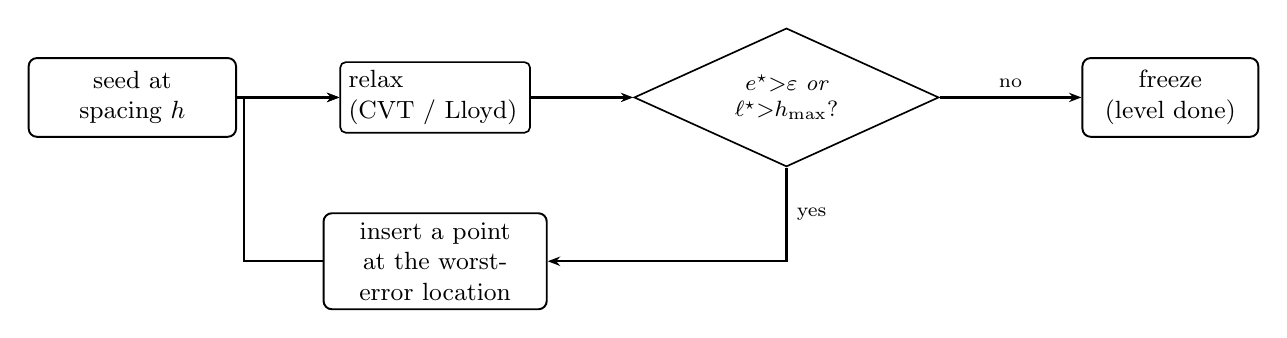
\begin{tikzpicture}[font=\small, node distance=7mm and 13mm]
 \node[rm stage, text width=24mm] (seed) {seed at spacing $h$};
 \node[rm state, text width=22mm, right=of seed] (relax) {relax\\(CVT / Lloyd)};
 \node[rm sel, aspect=2.2, text width=24mm, align=center, right=of relax] (dec)
   {$e^\star{>}\varepsilon$ \emph{or} $\ell^\star{>}h_{\max}$?};
 \node[rm out, text width=20mm, right=18mm of dec] (freeze) {freeze\\(level done)};
 \node[rm stage, text width=26mm, below=10mm of relax] (ins)
   {insert a point at the worst-error location};
 \draw[rm flow] (seed)--(relax);
 \draw[rm flow] (relax)--(dec);
 \draw[rm flow] (dec)--node[above,font=\scriptsize]{no} (freeze);
 \draw[rm flow] (dec.south) |- node[pos=0.25,right,font=\scriptsize]{yes} (ins.east);
 \draw[rm flow] (ins.west) -- ++(-10mm,0) |- (relax.west);
\end{tikzpicture}
\caption{The relax--insert--relax scheme shared by all stages
(\cref{prin:parallel}, mechanism (i)+(ii)). The error measure $e^\star$ is the
chord deflection (edges), the triangle--surface deflection (faces) or the
element quality (volume); $\ell^\star$ is the longest edge for the $h_{\max}$
bound. Iterate until both the tolerance and $h_{\max}$ hold and the sites stop
moving, then freeze.}
\label{fig:adaptive}
\end{figure}

\begin{algorithm}[H]
\caption{\textsc{MeshEdge}$(\vv{C},h,\varepsilon)$}
\label{alg:edge}
\KwIn{edge curve $\vv{C}$; sizing field $h$; deflection tolerance $\varepsilon$}
\KwOut{frozen edge points (corners included)}
tabulate $s(t)$; $L\gets s(t_1)$\;
$n \gets \max\bigl(1,\ \lceil \int_0^{L} h(s)^{-1}\dd s\rceil\bigr)$
   \tcp*{initial count from the sizing field}
place $s_1,\dots,s_n$ equidistributing $h$ (cumulative-$\rho$ inversion)\;
\Repeat{$e^\star\le\varepsilon$ \textbf{and} $\ell^\star\le h_{\max}$
        \textbf{and} max site move $<\tau_{\mathrm{move}}$}{
  \For{a few iterations}{relax all $s_i$ by \eqref{eq:cvt1d}\;}
  $e^\star,s^\star \gets$ worst chord--arc deflection and its location
     \tcp*{error-driven}
  $\ell^\star,m^\star \gets$ longest segment length and its midpoint
     \tcp*{$h_{\max}$-driven}
  \If{$e^\star>\varepsilon$ \textbf{or} $\ell^\star>h_{\max}$}{
     insert a site (at $s^\star$ if $e^\star{>}\varepsilon$, else $m^\star$);
     $n\mathrel{+}=1$\;
  }
}
\Return $\{\vv{C}(s_i)\}$\;
\end{algorithm}

\noindent
Shared edges are meshed once and cached, so both incident faces read identical
points, and all edges run in parallel (\cref{prin:parallel}).

% ============================================================================
\section{Stage 2: Faces}
\label{sec:faces}
% ============================================================================

A face is a trimmed surface $\vv{S}:\Omega\subset\R^2\to\R^3$, $(u,v)\mapsto
\vv{S}(u,v)$, bounded by oriented loops of frozen edges. The strategy is:
parameterise the face by a \emph{distance-faithful chart}, relax interior points
there with a 2D surface-CVT (boundary = frozen edge points, held fixed), insert
where the surface deflection tolerance is violated, and lift every chart point
exactly onto $\vv{S}$. The output is a \emph{conforming triangulation of the
face} that the volume stage will treat as a hard constraint.

\paragraph{Face categories and the face sizing field.}
Three chart families cover all modalities (\cref{sec:charts}): \emph{planar}
faces use the plane chart; \emph{developable} analytic faces (cylinder, cone,
extruded) use an exact isometric unroll; \emph{doubly-curved} analytic faces
(sphere, torus) and \emph{periodic} full revolutions use a distance-faithful
chart or the periodic revolution construction, with a restricted-CVT fallback
for general NURBS. Before any face is seeded, its sizing field is assembled from
the \emph{now-frozen edge sampling} on its boundary (the edge spacings and any
per-region $h_{\max}$) combined with the surface deflection bound
\eqref{eq:surf_defl}, then Lipschitz-smoothed \eqref{eq:lipschitz} across the
face. The frozen edges therefore both bound the face and seed its density.

\subsection{First fundamental form and area}
With $\Su=\partial\vv{S}/\partial u$, $\Sv=\partial\vv{S}/\partial v$, the metric
(first fundamental form) coefficients and area element are
\begin{equation}
\label{eq:fff}
E=\Su\!\cdot\!\Su,\quad F=\Su\!\cdot\!\Sv,\quad G=\Sv\!\cdot\!\Sv,
\qquad \dd A=\sqrt{EG-F^2}\;\dd u\dd v .
\end{equation}
A curve $t\mapsto(u(t),v(t))$ in parameter space has length
$\int\sqrt{E\dot u^2+2F\dot u\dot v+G\dot v^2}\,\dd t$; this is the metric the
chart must reproduce for Euclidean 2D operations (separation, centroid) to mean
arc length on the surface. \Cref{tab:geom} lists $E,F,G,\dd A$ for every analytic
modality, all derived with a computer-algebra system.

\paragraph{Worked example (sphere).}
For $\vv{S}(\lambda,\varphi)=r(\cos\varphi\cos\lambda,\cos\varphi\sin\lambda,
\sin\varphi)$,
\[
\Su=r(-\cos\varphi\sin\lambda,\ \cos\varphi\cos\lambda,\ 0),\qquad
\Sv=r(-\sin\varphi\cos\lambda,\ -\sin\varphi\sin\lambda,\ \cos\varphi),
\]
so $E=\Su\!\cdot\!\Su=r^2\cos^2\varphi$, $F=\Su\!\cdot\!\Sv=0$, $G=\Sv\!\cdot\!
\Sv=r^2$, giving $\dd A=r^2\abs{\cos\varphi}\dd\lambda\dd\varphi$ (the
$\cos\varphi$ is the polar foreshortening). With outward normal $\vv{n}=\vv{S}/r$
the second fundamental form is $L=\vv{S}_{\lambda\lambda}\!\cdot\!\vv{n}=
-r\cos^2\varphi$, $M=\vv{S}_{\lambda\varphi}\!\cdot\!\vv{n}=0$,
$N=\vv{S}_{\varphi\varphi}\!\cdot\!\vv{n}=-r$, hence the principal curvatures
$\kappa_1=L/E=-1/r$ and $\kappa_2=N/G=-1/r$ are equal (the sphere is umbilic) and
$K=\kappa_1\kappa_2=1/r^2$, the \cref{tab:geom} sphere row. The other rows
follow the same computation.

\begin{sidewaystable}\centering
\caption{Per-modality geometric quantities (all verified by computer algebra):
the parameterization $\vv{S}(u,v)$, the first fundamental form $E,F,G$ and area
element $\dd A$ (\cref{sec:faces}.1), and the Gaussian curvature $K$ and largest
principal curvature $\kappa_{\max}=1/R_{\min}$ that drive the deflection sizing
(\cref{sec:faces}.2). $\vv{a}$ is the unit axis, $\alpha$ the cone half-angle.
All but the NURBS row are diagonal ($F=0$); developables have $K=0$; the sphere
is umbilic.}
\label{tab:geom}
\small
\begin{tabularx}{\textheight}{@{}l L c c c L c L@{}}
\toprule
Surface & $\vv{S}(u,v)$ & $E$ & $F$ & $G$ & $\dd A$ & $K$ & $\kappa_{\max}=1/R_{\min}$\\
\midrule
Plane & $\vv{o}+u\vv{e}_1+v\vv{e}_2$ & $1$ & $0$ & $1$ & $\dd u\dd v$ & $0$ & $0$\\
Cylinder $(\theta,h)$ & $r(\cos\theta,\sin\theta)+h\vv{a}$ & $r^2$ & $0$ & $1$ & $r\,\dd u\dd v$ & $0$ & $1/r$\\
Sphere $(\lambda,\varphi)$ & $r(\cos\varphi\cos\lambda,\cos\varphi\sin\lambda,\sin\varphi)$ & $r^2\cos^2\varphi$ & $0$ & $r^2$ & $r^2\abs{\cos\varphi}\,\dd u\dd v$ & $1/r^2$ & $1/r$\\
Cone $(\theta,s)$ & $s\tan\!\alpha(\cos\theta,\sin\theta)+s\vv{a}$ & $s^2\tan^2\!\alpha$ & $0$ & $\sec^2\!\alpha$ & $\abs{s}\tan\!\alpha\sec\!\alpha\,\dd u\dd v$ & $0$ & $\dfrac{\cos\alpha}{s\tan\alpha}$\\[4pt]
Torus $(\theta,\phi)$ & $(R{+}r\cos\phi)(\cos\theta,\sin\theta){+}r\sin\phi\,\vv{a}$ & $(R{+}r\cos\phi)^2$ & $0$ & $r^2$ & $r\abs{R{+}r\cos\phi}\,\dd u\dd v$ & $\dfrac{\cos\phi}{r(R{+}r\cos\phi)}$ & $1/r$\\[4pt]
Extruded $(t,h)$ & $\vv{b}+P(t)+h\vv{a}$ & $\norm{P'(t)}^2$ & $0$ & $1$ & $\norm{P'(t)}\dd u\dd v$ & $0$ & $\dfrac{\abs{P'\times P''}}{\norm{P'}^3}$\\[4pt]
NURBS $(u,v)$ & tensor B-spline \cite{PieglTiller1997} & $\Su\!\cdot\!\Su$ & $\Su\!\cdot\!\Sv$ & $\Sv\!\cdot\!\Sv$ & $\sqrt{EG{-}F^2}$ & $\dfrac{LN{-}M^2}{EG{-}F^2}$ & $H{+}\sqrt{H^2{-}K}$\\
\bottomrule
\end{tabularx}
\end{sidewaystable}

\subsection{Curvature and surface deflection sizing}
The shape operator's eigenvalues are the principal curvatures
$\kappa_1,\kappa_2$; from the second fundamental form
$L=\vv{S}_{uu}\!\cdot\!\vv{n}$, $M=\vv{S}_{uv}\!\cdot\!\vv{n}$,
$N=\vv{S}_{vv}\!\cdot\!\vv{n}$ ($\vv{n}=\Su\times\Sv/\norm{\Su\times\Sv}$), the
Gaussian and mean curvatures are
\begin{equation}
\label{eq:KH}
K=\kappa_1\kappa_2=\frac{LN-M^2}{EG-F^2},\qquad
H=\tfrac12(\kappa_1+\kappa_2)=\frac{EN-2FM+GL}{2(EG-F^2)},
\end{equation}
and $\kappa_{1,2}=H\pm\sqrt{H^2-K}$. The per-modality values in \cref{tab:geom}
confirm the geometric intuition: developables have $K=0$ (cylinder, cone,
extruded), and the sphere is umbilic ($\kappa_1=\kappa_2=1/r$). For the cone the
single non-zero principal curvature is $\cos\alpha/(s\tan\alpha)$, growing
without bound toward the apex; for the torus the two principal curvatures are
$1/r$ (tube) and $\cos\phi/(R+r\cos\phi)$ (which changes sign across the
inner/outer equator), so $K$ is signed.

\noindent
The surface sagitta argument mirrors \eqref{eq:sagitta} with $R=R_{\min}=
1/\kappa_{\max}$: a triangle edge of length $\ell$ on a surface of smallest
principal radius $R_{\min}$ deviates from the surface by
$\varepsilon\approx \ell^2/(8R_{\min})$, so the face sizing field is
\begin{equation}
\label{eq:surf_defl}
h_{\text{face}}(\vv{x}) \;=\;
\min\!\Bigl(h_{\max},\ \sqrt{8\,\varepsilon\,R_{\min}(\vv{x})}\Bigr),
\qquad R_{\min}=1/\kappa_{\max}.
\end{equation}

\subsection{Distance-faithful charts}
\label{sec:charts}
A chart $\Phi:\,\text{face}\to\R^2$ lets the planar CVT machinery act on the
surface (\cref{fig:chart}). We want $\Phi$ as close to an \emph{isometry} as
possible so Euclidean 2D distance equals surface arc length.

\begin{figure}[H]\centering
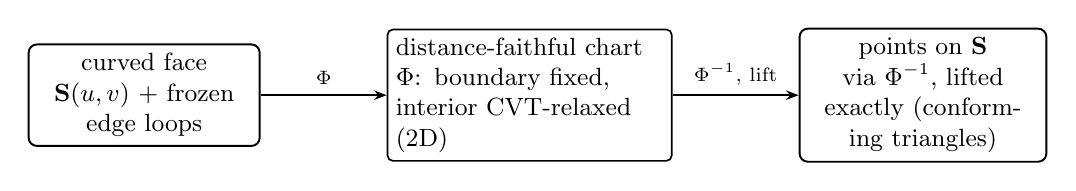
\begin{tikzpicture}[font=\small, node distance=16mm]
 \node[rm stage, text width=27mm] (S) {curved face $\vv{S}(u,v)$ $+$ frozen edge loops};
 \node[rm state, text width=34mm, right=of S] (chart)
   {distance-faithful chart $\Phi$: boundary fixed, interior CVT-relaxed (2D)};
 \node[rm out, text width=29mm, right=of chart] (lift)
   {points on $\vv{S}$ via $\Phi^{-1}$, lifted exactly (conforming triangles)};
 \draw[rm flow] (S)--node[above,font=\scriptsize]{$\Phi$} (chart);
 \draw[rm flow] (chart)--node[above,font=\scriptsize]{$\Phi^{-1}$, lift} (lift);
\end{tikzpicture}
\caption{Surface meshing through a chart: relax in a (near-)isometric 2D
parameterization with the frozen edge points as fixed boundary, then lift every
chart point back onto the analytic surface. Exact on developables, bounded
distortion on the sphere (\cref{eq:azeq}).}
\label{fig:chart}
\end{figure}

\paragraph{Developables (cylinder, cone, extruded): exact isometry.}
A surface with $K\equiv0$ unrolls into the plane without distortion.
\begin{itemize}[topsep=2pt,itemsep=1pt]
\item \emph{Cylinder}: $\Phi(\theta,h)=(r\theta,\ h)$. Then $E=G=1,F=0$ in the
chart, exact.
\item \emph{Cone}: polar unroll $\Phi(\theta,s)=\bigl(\rho\cos\psi,\rho\sin\psi
\bigr)$ with slant $\rho=s/\cos\alpha$ and sweep $\psi=\theta\sin\alpha$. The
induced chart metric is $E=s^2\tan^2\alpha,\ F=0,\ G=\sec^2\alpha$, identical
to the cone's first fundamental form (\cref{tab:geom}), i.e.\ \emph{exactly
isometric}.
\item \emph{Extruded}: $\Phi(t,h)=(\sigma(t),\,h)$ with $\sigma(t)=\int^t\norm
{P'}$ the profile arc length; $E=G=1,F=0$, exact.
\end{itemize}

\paragraph{Sphere: azimuthal-equidistant.}
The sphere ($K=1/r^2\neq0$) admits no isometry to the plane. We use the
azimuthal-equidistant chart about a cap centre: the chart radial coordinate is
the exact geodesic distance $r\psi$ ($\psi$ the geodesic colatitude), so radial
distances are exact; the circumferential direction stretches by
\begin{equation}
\label{eq:azeq}
\text{stretch}(\psi)=\frac{\psi}{\sin\psi}
   = 1+\frac{\psi^2}{6}+\frac{7\psi^4}{360}+O(\psi^6),
\end{equation}
which is $\le 1.05$ for caps up to $\psi\approx 32^\circ$ and stays bounded
well past a hemisphere. The chart is a bijection on any cap that excludes the
antipode; bijectivity is validated by a round-trip test
$\dist\!\bigl(\proj_{\vv{S}}(\vv{p}),\,\Phi^{-1}\Phi(\vv{p})\bigr)<\text{tol}$.

\paragraph{Forward and inverse maps.}
Each chart provides $\Phi$ (surface point $\to$ chart, to place the fixed
boundary) and $\Phi^{-1}$ (chart $\to$ surface, to lift relaxed interior points):
\begin{align}
\label{eq:chartmaps}
\text{cylinder}&: & \Phi(\theta,h)&=(r\theta,h), &
   \Phi^{-1}(x,y)&=\vv{S}\bigl(x/r,\,y\bigr);\notag\\
\text{cone}&: & \Phi(\theta,s)&=\tfrac{s}{\cos\alpha}(\cos\psi,\sin\psi),\
   \psi=\theta\sin\alpha, &
   \Phi^{-1}(x,y)&=\vv{S}\!\Bigl(\tfrac{\operatorname{atan2}(y,x)}{\sin\alpha},\,
     \cos\alpha\sqrt{x^2{+}y^2}\Bigr);\\
\text{extruded}&: & \Phi(t,h)&=(\sigma(t),h), &
   \Phi^{-1}(x,y)&=\vv{S}\bigl(\sigma^{-1}(x),\,y\bigr);\notag\\
\text{sphere}&: & \Phi&=\log_{\vv c},\ \Phi^{-1}=\exp_{\vv c}
   &&\text{(geodesic polar about $\vv c$).}\notag
\end{align}
For the sphere, $\log_{\vv c}(\vv{p})$ returns the chart point at radius $r\psi$
($\psi=\arccos(\hat{\vv c}\!\cdot\!\hat{\vv p})$ the geodesic colatitude) along
the bearing of the tangent toward $\vv{p}$; $\exp_{\vv c}(\vv{u})$ walks the
geodesic of length $\norm{\vv{u}}$ from $\vv c$. The extruded $\sigma^{-1}$ is
the arc-length table inversion of \cref{sec:edges}.1. Every lift lands
\emph{exactly} on the analytic surface, so the resulting boundary vertices
satisfy the same on-surface guarantee as an explicit closest-point projection.

\paragraph{General NURBS / non-developable: metric-scaled or restricted CVT.}
For a NURBS patch we scale the parameters by the local metric
$(\sqrt{E},\sqrt{G})$ at the patch centroid (a first-order isometry) and, when a
single chart distorts too much, fall back to a genuine restricted-Voronoi
relaxation on the surface \cite{YanLevy2009,LevyLiu2010}: the centroid
\eqref{eq:disc_centroid} is computed from the restricted cells and the move is
projected back onto $\vv{S}$ by closest-point.

\paragraph{Revolution faces and periodicity.}
A full revolution (cylinder/cone/torus barrel) is periodic in $\theta$; its
boundary loops are rim circles that do not close in the unrolled rectangle.
Such a face is meshed by a structured $(\theta,v)$ grid whose rings reuse the
\emph{rim} longitudes (radial alignment, no seam) and whose row spacing follows
$h$ in arc length; the uniform grid is the on-surface CVT optimum of a
developable. A sphere cap meeting an intersection circle is itself a revolution
about the line of centres (the circle lies in a plane $\perp$ that axis), so the
same latitude/longitude construction applies, with both incident caps deriving
their longitude reference from the \emph{shared} rim so their rings align.

\begin{algorithm}[H]
\caption{\textsc{BuildChart}$(\vv{S},\,\text{verts})$}
\label{alg:chart}
\KwIn{analytic surface $\vv{S}$; representative on-surface points of the face}
\KwOut{chart $(\Phi,\Phi^{-1})$, or \textsc{None} (caller falls back)}
\Switch{kind of $\vv{S}$}{
  \uCase{plane}{$(\Phi,\Phi^{-1})\gets$ in-plane orthonormal frame}
  \uCase{cylinder / cone / extruded}{$(\Phi,\Phi^{-1})\gets$ exact isometric
     unroll \eqref{eq:chartmaps}}
  \uCase{sphere}{$\vv c\gets$ projected centroid of verts;
     $(\Phi,\Phi^{-1})\gets(\log_{\vv c},\exp_{\vv c})$}
  \Other{metric-scale the parameters by $(\sqrt E,\sqrt G)$ at the centroid}
}
\If{$\max_{\text{verts}}\dist\!\bigl(\proj_{\vv S}(\vv p),\,\Phi^{-1}\Phi(\vv p)
     \bigr)>\mathrm{tol}$}{
   \Return \textsc{None} \hfill\tcp*[h]{wrapping/closed $\to$ revolution grid}}
\Return $(\Phi,\Phi^{-1})$\;
\end{algorithm}

\begin{algorithm}[H]
\caption{\textsc{RevolutionGrid}$(\vv{S},\vv a,\text{rim loops},h)$}
\label{alg:rev}
\KwIn{revolution surface $\vv{S}$; axis $\vv a$; rim edge points; field $h$}
\KwOut{interior surface points (seam-free, rim-aligned)}
$\{\theta_k\}\gets$ longitudes of the rim points about $\vv a$ (sorted, dedup)
   \hfill\tcp*[h]{shared by both incident faces}\;
$[v_0,v_1]\gets$ the $v$-extent of the rim loops\;
$n_v\gets\max\!\bigl(1,\lceil\operatorname{arclen}(v_0,v_1)/h\rceil\bigr)$\;
\For{interior row $j=1,\dots,n_v-1$}{
  $v_j\gets v_0+(v_1-v_0)\,j/n_v$\;
  \For{each $\theta_k$ \normalfont(thinned by $\cos$ toward a pole)}{
     emit $\vv{S}(\theta_k,v_j)$ \hfill\tcp*[h]{ring aligned to the rim}}}
\Return the interior rings \hfill\tcp*[h]{rims/poles are the shared edges}\;
\end{algorithm}

\subsection{Surface CVT and adaptivity}
\begin{algorithm}[H]
\caption{\textsc{MeshFace}$(\vv{S},\text{loops},h,\varepsilon)$}
\label{alg:face}
\KwIn{trimmed surface $\vv{S}$; frozen boundary loops; field $h$; tolerance $\varepsilon$}
\KwOut{conforming triangulation of the face (triangles + on-surface vertices)}
build chart $\Phi$ (modality-driven); validate bijectivity\;
$B \gets \Phi(\text{frozen edge points of all loops})$ \tcp*{fixed boundary in chart}
scatter interior sites in $\Phi(\text{face})$ at spacing $h$ (greedy graded Poisson)
   inside the trim loops\;
\Repeat{$e^\star\le\varepsilon$ \textbf{and} $\ell^\star\le h_{\max}$
        \textbf{and} max move $<\tau_{\mathrm{move}}$}{
  \For{a few iterations}{
     2D Delaunay of $B\cup\{\text{interior}\}$ (exact predicates)\;
     move each interior site by \eqref{eq:disc_centroid}, $\rho=h^{-2}$,
        clamp inside the loops; keep $B$ fixed\;
  }
  $e^\star \gets \max$ triangle deflection vs.\ $\vv{S}$ (sagitta,
     \eqref{eq:surf_defl}) \tcp*{error-driven}
  $\ell^\star \gets \max$ triangle edge length (arc length) \tcp*{$h_{\max}$-driven}
  \If{$e^\star>\varepsilon$ \textbf{or} $\ell^\star>h_{\max}$}{
     insert a site at the offending triangle's circumcentre (in the chart)\;
  }
}
lift $\vv{p}_k=\vv{S}(\Phi^{-1}(\text{chart site}_k))$, exact on surface\;
\Return triangulation\;
\end{algorithm}

\noindent
After Stage 2 every face carries a frozen, conforming triangulation; shared
edges guarantee face-to-face conformity, and all faces run in parallel
(\cref{prin:parallel}). The union of all face triangulations is a watertight
surface mesh $\mathcal{S}$.

% ============================================================================
\section{Stage 3: Volume}
\label{sec:volume}
% ============================================================================

\subsection{Sizing field from the surface}
The volume field is the same gradient-limited sizing field (\eqref{eq:lipschitz})
carried into the interior, with the \emph{final} surface vertices as its sources
--- each contributing its local surface element size --- so it already reflects
the curvature- and feature-driven refinement of the completed surface. It is
capped per region by the region's own \code{maxh} and by the global
\code{maxh\_vol}, and is queried from an octree of the surface points so distant
sources cost nothing. A region whose walls come close (a thin web, a slender bore
wall) is therefore resolved wherever the surface there was already refined.

\subsection{Interior seeding}
Interior sites are placed on a graded lattice at the local field density: a
regular grid at step $\approx h$ is walked, and a candidate is kept only if it
lies inside the region, is at least one local element clear of the surface (a
closer seed would force a tetrahedron the constrained build cannot emit), and is
not within $0.6\,h$ of an already-accepted site (a spatial-hash separation
guard). Surface vertices are \emph{not} re-seeded; they are the fixed boundary of
the volume point set.

\subsection{ODT relaxation and quality-driven adaptivity}
Interior sites relax by the optimal-Delaunay update \eqref{eq:odt} on an
\emph{unconstrained} Delaunay rebuilt each pass; the surface vertices stay fixed,
and a relocation that would leave the domain or come within a local element of the
surface is rejected (the site keeps its position). After a pass, sites are
inserted at the longest edge of any tetrahedron coarser than the field, and the
relaxation continues. The loop terminates adaptively --- once the layout has
settled (maximum move below a fraction of the spacing) \emph{and} seeding has
stopped, or once the in-domain sliver count has plateaued --- under a hard pass
cap; the boundary-constrained build below then runs once.

\subsection{Boundary-constrained tetrahedralization}
The volume is the \emph{constrained
Delaunay tetrahedralization} (CDT) of the interior sites \emph{plus} the frozen
surface mesh $\mathcal{S}$ as constraint facets
\cite{Si2015,ShewchukCDT2002,ChengDeyShewchuk2012}:
\begin{equation}
\text{Tetrahedralize}\bigl(\{\text{interior sites}\}\cup V(\mathcal{S})\bigr)
\quad\text{s.t. every } \triangle\in\mathcal{S} \text{ is a union of tet faces.}
\end{equation}
Because $\mathcal{S}$ is watertight and every constraint triangle is recovered
as tetrahedron faces, each surface triangle has a tetrahedron exactly on each
side; region labels are then assigned by flood fill across non-constraint faces
starting from the region tag attached to each surface triangle's two sides.
No tetrahedron straddles the boundary, so:

\medskip
\noindent
\emph{Per-region parallelism.} Each material region is bounded by a disjoint
subset of the frozen $\mathcal{S}$ (its outer walls and the interface facets it
shares with neighbours, all read-only), so the regions' constrained
tetrahedralizations are independent and run in parallel
(\cref{prin:parallel}); a shared interface facet is meshed once on $\mathcal{S}$
and both regions tetrahedralize against the same fixed triangles, which keeps
the multi-material mesh conforming across interfaces.

\begin{proposition}[Watertightness]
\label{prop:watertight}
If $\mathcal{S}$ is a closed, non-self-intersecting, conforming surface mesh and
the CDT recovers it, then $\mathcal{S}$ is covered by tet faces with exactly one
tetrahedron on each side (a planar facet may be re-triangulated within its own
plane, which leaves the surface geometry unchanged), each side carrying the
region label prescribed by $\mathcal{S}$, and the boundary of each meshed region
is exactly the corresponding subset of $\mathcal{S}$. In particular there are no
protrusions into a void and no gaps.
\end{proposition}

\noindent
The constraint is honoured \emph{without} a separate facet-recovery search. A
surface vertex is inserted exactly on its carrier (a point on a line, $\vv x=\vv
a+t(\vv b-\vv a)$, or on a plane, $\vv x=\vv a+u(\vv b-\vv a)+v(\vv c-\vv a)$, so
it stays exactly on the carrier under any later split). \emph{Planar facets then
need no recovery}: their vertices are coplanar, so the Delaunay restricted to the
plane already tiles them with a tetrahedron on each side, leaving a planar
region's volume bit-exact. Curved facets are \emph{not} force-recovered---a chosen
curved triangulation is in general far from Delaunay, so forcing it would need
unbounded Steiner insertion, and the chord is a tolerance approximation anyway
(\cref{sec:errctl}). Instead a multi-material scene is decomposed \emph{per
region} (\cref{alg:region}): each region is tetrahedralized independently against
its own subset of the frozen surface, and every tetrahedron whose centroid does
not classify into that region by the exact inside predicate is discarded, so no
tetrahedron straddles a region interface; the shared interface vertices (one
global index per vertex) keep adjacent regions conforming. A single-region body
is the constrained Delaunay of its frozen surface directly. The curved boundary
of a region is thus the restricted Delaunay of its frozen-surface points,
watertight by \cref{prop:watertight} and free of straddlers by construction.

\begin{algorithm}[H]
\caption{\textsc{MeshRegion}$(\mathcal{S},r,\text{interior})$: per-region
constrained fill (straddler-free by construction)}
\label{alg:region}
\KwIn{frozen surface $\mathcal{S}$ (region-tagged); region $r$; interior sites}
\KwOut{tetrahedra of region $r$, conforming on shared interfaces}
$F_r\gets\{\triangle\in\mathcal{S}: r\in\operatorname{regions}(\triangle)\}$
   \hfill\tcp*[h]{outer walls $+$ interfaces bounding $r$}\;
$V_r\gets$ vertices of $F_r$ (exact on carriers) $\cup\;
   \{\,p\in\text{interior}:\operatorname{region}(p)=r\,\}$\;
$\mathcal{T}_r\gets$ constrained Delaunay of $V_r$ with $F_r$ as planar
   constraints\;
\lForEach{$t\in\mathcal{T}_r$}{%
   \lIf{$\operatorname{region}(\operatorname{centroid}t)\ne r$}{discard $t$}}
\Return the kept tetrahedra, tagged $r$
   \hfill\tcp*[h]{interface verts shared by global index $\Rightarrow$ conforming}\;
\end{algorithm}

\paragraph{Quality measures and the cleanup pass.}
Element quality is reported as the minimum dihedral angle and the
\emph{radius--edge ratio} $\rho=R_{\text{circ}}/\ell_{\min}$; Delaunay refinement
bounds $\rho$, but \emph{slivers} (near-zero volume, dihedral $\to0$, yet
acceptable $\rho$) can survive and are the residual enemy. They are removed by a
conformity-preserving post-pass that leaves $\mathcal{S}$ and the region partition
intact: \emph{(i)} smoothing each free vertex toward its quality-weighted optimum,
boundary vertices only \emph{within their surface/edge carrier} (a tangential move
that, to first order, leaves each region's enclosed volume unchanged and keeps
interface vertices exactly on their analytic carrier); \emph{(ii)} topological
operations --- $2$--$3$ face flips and an edge removal that re-triangulates the
$k$-tetrahedron ring around an interior edge by the dynamic program maximising its
worst dihedral; and \emph{(iii)} a dedicated sliver stage that, for an interior
sliver, inserts a vertex whose position a pattern search drives to maximise the
worst cone dihedral (a local perturbation), and, for a boundary sliver whose
vertices are all pinned, splits the offending surface face $1$--$3$ at a Steiner
point \emph{on} the analytic carrier (so \cref{prop:watertight} is preserved).
Each accepted operation strictly improves the local worst dihedral
\cite{TournoisAlliez2009,AlliezCohenSteiner2005}.

\begin{algorithm}[H]
\caption{\textsc{MeshVolume}$(\mathcal{S},h)$}
\label{alg:vol}
\KwIn{watertight surface mesh $\mathcal{S}$ (with region tags); field $h$}
\KwOut{tetrahedra, per-tet region, boundary faces ($=\mathcal{S}$)}
build $h_{\text{vol}}$ from $\mathcal{S}$ (surface sources, gradation-limit
   \eqref{eq:lipschitz}, per-region cap)\;
seed interior sites on a graded lattice, clearance $\ge h$ from $\mathcal{S}$\;
\Repeat{layout settled \textbf{and} no insertion, \textbf{or} slivers plateaued}{
  \emph{unconstrained} Delaunay of $(\text{interior}\cup V(\mathcal{S}))$\;
  relax interior sites by the ODT update \eqref{eq:odt} (surface vertices fixed)\;
  insert a site at the longest edge of any tetrahedron coarser than the field\;
}
\lForEach{region $r$}{\textsc{MeshRegion}$(\mathcal{S},r,\text{interior})$
   \tcp*[h]{\cref{alg:region}: constrained, straddler-free}}
assign per-tet region tags; quality $+$ sliver post-pass (carrier-constrained)\;
\Return tetrahedra, per-tet region, boundary faces ($=\mathcal{S}$)\;
\end{algorithm}

% ============================================================================
\section{The sizing field, end to end}
% ============================================================================
The single field $h$ threads all stages and is only ever \emph{refined}
downward in size:
\begin{enumerate}[topsep=2pt,itemsep=1pt]
\item \textbf{Edges} set $h$ from curve deflection \eqref{eq:edge_h} and
$h_{\max}$ / per-region overrides.
\item \textbf{Faces} take the min of the edge field and the surface deflection
bound \eqref{eq:surf_defl}; the smoothed result drives the surface CVT.
\item \textbf{Volume} carries the face field into the interior from the surface
vertices as sources, capped per region, then gradation-limits
\eqref{eq:lipschitz} through the interior.
\end{enumerate}
Because each stage only ever lowers $h$ and then re-smooths, the field is
monotone and Lipschitz, and the element-size contract (a documented
$1.5\times$ max-edge bound, as in gmsh) holds globally.

\subsection{Error control: two orthogonal axes}
\label{sec:errctl}
The user controls the mesh through two \emph{independent} kinds of bound, which
must not be conflated.
\begin{description}[topsep=2pt,itemsep=2pt,leftmargin=1.4em]
\item[Conformity] (exact). The meshed region fills exactly the volume enclosed
by the frozen surface mesh: there are no straddling tetrahedra
(\cref{prop:watertight}). This is not a tunable tolerance; it is a structural
guarantee, verified to machine-rational equality on planar fixtures
(\cref{sec:validation}). It says nothing about how well the surface mesh
approximates a \emph{round} geometry.
\item[Geometric accuracy] (a relative tolerance). How closely the piecewise-linear
surface follows the true analytic geometry, governed by the deflection bounds
$\varepsilon_{\text{edge}}=$\code{tol\_edge} and $\varepsilon_{\text{surf}}=$\code{tol\_surf}.
By \eqref{eq:defl_len}/\eqref{eq:surf_defl} an entity of principal radius $R$ is
sized $h=R\sqrt{8\varepsilon}$, so the chord deviates by at most $\varepsilon R$
(\emph{relative}, hence scale-invariant). The default $\varepsilon=10^{-2}$
($1\%$) is a good engineering mesh; $10^{-4}$ is very fine. A round surface is
never meshed exactly, so a conformity demand of $10^{-9}$ on a curved body is a
category error: it is the \emph{fill} that is exact, not the chord.
\end{description}

\paragraph{Size and tolerance handles.}
Element size is capped per dimension by \code{maxh\_edge}, \code{maxh\_surf},
\code{maxh\_vol}, each combined with the global \code{maxh} as the minimum; there
is no volume \emph{tolerance} (the volume size follows from the surface,
\cref{sec:volume}). Every bound is settable per individual entity through a
\emph{hierarchical} handle that mirrors the dimensional hierarchy
(\cref{prin:parallel}):
\begin{center}
\code{g.region(sel).surf(sel).edge(sel).maxh}\quad/\quad\code{.tol}
\end{center}
A level addressed without a selector applies to all of its children
(\code{g.edge().tol} sets every edge, i.e.\ the global \code{tol\_edge};
\code{g.maxh} sets everything), and a selector (\code{tag}, \code{normal},
\code{near}, \code{between}) narrows it to specific entities. Resolution is
most-specific-wins: a per-entity override beats the per-dimension default, which
beats the global. The selectors are resolved against the B-rep topology (region
$\to$ faces $\to$ edges, \cref{sec:booleans}), so the same composition that
structures the algorithm structures its control surface; power users drive local
refinement (a boundary layer on one face, a fine seam on one edge) without a
separate selection language.

% ============================================================================
\section{Complexity and parallel scaling}
% ============================================================================
Let $N$ be the output vertex count. Every stage is dominated by an incremental
Delaunay or a fast-marching sweep, each $O(N\log N)$ with exact predicates: the
gradation field \eqref{eq:gradenvelope} by heap fast-marching (\cref{alg:grad}),
the surface/volume triangulations by Bowyer--Watson with octree-accelerated point
location. The variational relaxation is a fixed number of passes, each a rebuilt Delaunay
plus a linear sweep (the centroid move \eqref{eq:disc_centroid} on edges and
faces, the ODT move \eqref{eq:odt} in the volume);
because the sites are already near-uniform and the per-region constrained fill
(\cref{alg:region}) carries no facet-recovery search, the dominant cost is the
constrained Delaunay itself, and slivers left for the cleanup pass are rare
\cite{AlliezCohenSteiner2005,TournoisAlliez2009}.

The structure is what makes it scale. Within a level the entities are independent
(\cref{prin:parallel}), so with $P$ workers the wall-clock of a stage is the
\emph{slowest single} edge / face / region, not their sum; the only global
synchronisations are the two barriers between the three stages. Multi-region and
boolean-heavy scenes parallelise for free over regions, since each region's
constrained tetrahedralization is independent and shares only read-only interface
facets. All relaxation queries are local (octree neighbours), so memory and the
per-pass cost stay $O(N)$.

% ============================================================================
\section{Why this guarantees conformity}
\label{sec:conformity}
% ============================================================================
The natural alternative (a single \emph{unconstrained} Delaunay over all
points, with each tetrahedron labelled by the region of its centroid) recovers
the boundary only \emph{statistically}: where the surface sample is coarser than
a feature, a tetrahedron straddles the true surface, and whole-tet labelling then
produces a protrusion (centroid inside) or a gap (centroid outside). The
algorithm specified here removes that failure mode at its root by (a) completing
a watertight, error-controlled surface mesh \emph{first}, and (b) making that
mesh a \emph{constraint} on the volume rather than a target to be rediscovered.
Conformity is then a theorem
(\cref{prop:watertight}), not a sampling-density gamble. The cost is the
constrained Delaunay / facet recovery, which is exactly the machinery the method
must keep; the variational (CVT) relaxation supplies the well-shaped interior
that keeps recovery cheap and slivers rare
\cite{AlliezCohenSteiner2005,TournoisAlliez2009}.

% ============================================================================
\section{Surface meshing and adaptivity}
\label{sec:surface}
% ============================================================================
The same machinery also runs as a \emph{standalone surface mesher}: the planar
surface stage (\cref{sec:faces}) exported on its own, with no volume, as the 2D
product an electromagnetic surface solver (method-of-moments, 2D FEM) consumes.
Here quality is the deliverable rather than a by-product of the volume constraint,
so the planar patches are triangulated by a guaranteed-quality Delaunay refinement
in place of the fixed-pass CVT.

\subsection{Sliver-free Ruppert/Chew refinement}
Each planar patch is refined by a sizing-field-driven Ruppert/Chew loop
\cite{Ruppert1995,Chew1993}: a triangle whose circumradius-to-shortest-edge ratio
exceeds the bound (equivalently, whose smallest angle is below the target) has its
circumcenter inserted; a boundary segment encroached by such an insertion is split
at its midpoint instead. The loop terminates with a guaranteed \emph{minimum
angle} --- the implementation targets $20^\circ$ --- so the output is
\emph{sliver-free at any density}, and no triangle exceeds the local sizing target
$h(\vv{x})$, so the mesh grades smoothly. An apex-indexed encroachment test and a
hash-grid spacing guard keep the refinement near-linear (the two quadratic costs of
a naive Ruppert removed).

A \emph{boundary-preserving} optimal-Delaunay (ODT) smoothing then equalises the
interior: each free vertex moves toward the area-weighted ODT target
\eqref{eq:odt}, under-relaxed, with the boundary frozen and a per-pass guard that
reverts any pass which would drop the global minimum angle below the bound. This
keeps the Ruppert guarantee while removing the density jump a bare refinement
leaves just inside the boundary.

\subsection{Element and triangle budgets}
\label{sec:budget}
Both meshers take an optional \emph{budget}. \code{mesh(target\_elements=$N$)}
retunes the single global size scale over a few remeshes: because the element
count scales as $\mathrm{scale}^{-3}$, each step multiplies the scale by
$(n/N)^{1/3}$, so the final count lands within a few percent of $N$ while the
\emph{relative} refinement (curvature, size points) keeps its shape.
\code{surface\_mesh(target\_triangles=$N$)} is instead a \emph{cap}: the
count-driven Ruppert resolves the field down to its floor $h_{\min}$ but stops once
the triangle count reaches $N$ (the budget split across patches by area), spending
its last splits on the worst-quality triangles. One mesh therefore yields
$\min(\text{field-resolved},\,\text{budget})$, still graded and sliver-free.

\subsection{Adaptive refinement (D\"orfler marking)}
\label{sec:amr}
The surface mesher closes the \textsc{mark}\,$\to$\,\textsc{refine} half of an
adaptive loop; \textsc{solve} and \textsc{estimate} belong to the solver. Given a
per-triangle error indicator $\eta_t$ (an a-posteriori estimator, e.g.\
$\mathrm{area}\cdot\lvert\nabla u\rvert$), \emph{D\"orfler bulk marking}
\cite{Doerfler1996} selects the smallest element set $\mathcal{M}$ whose summed
\emph{squared} indicator reaches a fraction $\theta$ of the total,
\begin{equation}
  \sum_{t\in\mathcal{M}} \eta_t^2 \;\ge\; \theta \sum_t \eta_t^2,
  \qquad \theta\in(0,1]\ (\text{default }0.5),
  \label{eq:dorfler}
\end{equation}
the energy-norm convention. Each marked element becomes a \emph{point size source}
at $h_{\text{local}}/\text{factor}$ (clamped to $h_{\min}$): the mesher's
gradient-limited grading spreads it into a smooth background field and the Ruppert
refinement re-triangulates, so \emph{every adapted mesh stays sliver-free} with the
same guaranteed minimum angle. One \textsc{estimate}\,$\to$\,\textsc{mark}\,$\to$%
\,\textsc{refine} step is \code{refine\_dorfler}; iterated, it concentrates
resolution where the error lives.

The indicator must be a \emph{proper} a-posteriori estimator --- the per-element
error, which \emph{shrinks} as an element refines ($\eta\sim h^k$). Then
$\mathcal{M}$ stays small and the loop converges. A pointwise field that does
\emph{not} shrink on refinement (a bare $e^{-r^2}$, say) makes D\"orfler re-mark the
same region every pass, so the refinement never localises --- it ``refines
everywhere'', the failure the squared-indicator marking exists to avoid.

% ============================================================================
\section{FEM and MoM export}
\label{sec:export}
% ============================================================================
Because the mesher is a pure-Rust library, its meshes are consumed in-process by
sibling Rust solvers (the method-of-moments code \textsf{rapidmom} bundles
\code{rapidmesh-tet} as a crate). Beyond the raw points and triangles, the surface
mesh exposes the derived connectivity a surface solver would otherwise rebuild
(\code{rapidmesh\_tet::mom}):
\begin{itemize}[nosep,leftmargin=1.4em]
  \item \emph{edge adjacency} --- each undirected edge mapped to its up-to-two
        incident triangles and their conductor tags;
  \item \emph{RWG basis edges} --- the surface degrees of freedom: interior edges
        shared by two triangles of the \emph{same} conductor, returned as
        $[v_0,v_1,t_+,t_-]$ with the current orientation $+\!\to\!-$;
  \item the \emph{conductor outline} (boundary edges --- a free side or a tag
        change) and \emph{port edges} (boundary edges on a query line), the
        excitation the solver feeds;
  \item per-triangle \emph{area} and \emph{minimum angle}, the element-quality
        field (all $\ge$ the Ruppert bound).
\end{itemize}
These are computed natively and validated bit-identical to a reference NumPy
implementation, so a Rust solver drives the whole mesh\,$\to$\,assemble pipeline
with no Python in the loop.

\paragraph{Hierarchical per-entity sizing.}
The geometry API exposes a fluent selector,
\code{g.region($s$).surf($s$).edge($s$).maxh}\,/\,\code{.tol}, that resolves a
scope to B-rep entity ids natively (\code{rapidmesh\_brep::Topology}): a region by
tag, a face by tag/normal/proximity, an edge by its bounding regions, kind, or
proximity. A bare dimension scope (\code{g.surf().maxh}) sets the global
per-dimension target; a filtered scope sets the per-entity overrides the sizing
field then honours, so a single curved face or one conductor edge is refined
without touching the rest.

% ============================================================================
\section{Validation}
\label{sec:validation}
% ============================================================================
The algorithm is validated on a from-scratch corpus of ninety-five geometries
generated directly through the geometry API (no pre-baked tessellations), spanning
nine families: \emph{2D plates} (the planar surface stage in isolation),
\emph{analytic primitives}, \emph{CSG booleans} and multi-region assemblies,
hierarchical \emph{sizing} and \emph{gradation} cases, parametric \emph{shape}
sweeps, \emph{showcase} models, \emph{RF/EM} structures, and \emph{passives}
(method-of-moments spiral inductors and transformers, meshed as surfaces). Each geometry is
meshed at its default density and rendered headlessly by the project's WebGPU
rasterizer --- which runs the \emph{same} scene pipeline as the live viewer, with
no browser --- into a \textsc{normal} view (region-coloured, volumes clipped to
expose the interior) and a \textsc{debug} view that overlays the located defect
markers and the per-stage meshing time. The full per-geometry metric set (point
and element counts, minimum dihedral angle, watertightness, sliver / straddler /
non-manifold-edge counts, maximum surface deviation) is tabulated per family in
the longtables below, and every mesh is shown in the gallery at the end of this
section.

\medskip\noindent
\textbf{Summary.} 93 of 95 geometries mesh (two RF/passives assemblies are
degenerate inputs). Of the 72 volume meshes, 48 are watertight and 40 are free of
slivers and straddlers; the analytic-primitive and box-derived (sizing, gradation)
families are watertight and sliver-free at the expected isotropic quality (minimum
dihedral typically $12$--$20^\circ$). On the harder
curved-boolean, showcase and RF families watertightness is \emph{partial}: the
residual failures concentrate on \emph{curved material interfaces} --- where a
chosen curved-facet triangulation is not force-recovered (\cref{sec:volume}) ---
and on dense multi-region assemblies, with a few revolution apices and thin tubes
retaining slivers the cleanup pass does not fully clear. These are the standing
open items the corpus exists to track. Conformity on planar and single-curved
geometry is exact by \cref{prop:watertight} and independent of density: the
boundary-constrained, per-region tetrahedralization (\cref{alg:region}) makes the
frozen surface a hard constraint and discards every straddling tetrahedron, so a
region's boundary is exactly the prescribed subset of $\mathcal{S}$. The
validation harness (\code{report/corpus.py}, \code{report/render\_gallery.py})
re-runs the whole matrix and regenerates these tables and figures on demand, so
the corpus is a standing regression gate.

\input{generated/metrics.tex}

\subsection{Gallery}
\label{sec:gallery}
A representative geometry or two from each family; the \textsc{normal} view (left:
region-coloured solid, volumes clipped in $y$ to expose the interior tetrahedra)
sits beside the \textsc{debug} view (right: surface wireframe, located defect
markers, and a metrics + meshing-time overlay). The full per-geometry metric set
for the entire corpus is in the longtables above.
\input{generated/gallery.tex}

\printbibliography[title={References}, heading=bibintoc]

\end{document}
